%
% Pre-installed VMs
%

\chapter{Pre-installed virtual machines}
\label{vms}

Since not everybody is willing to install {\em pDLNA} on a system, just to verify if {\em pDLNA} fulfills his needs or just likes to test {\em pDLNA} for the first time, there are some pre-installed virtual machines available to download from the {\em pDLNA} website available under the following URL: \url{www.pdlna.org/cgi-bin/index.pl?menu=vm}

\begin{colframeimportantnote}
\textsc{IMPORTANT NOTE:} These pre-installed virtual machines are prepared to have a quick look on {\em pDLNA} and are not designed to be used in a productive environment or for any other purpose.
\end{colframeimportantnote}

These virtual machines are provided in the {\em Open Virtualization Format} (OVF)\footnote{\url{http://en.wikipedia.org/wiki/Open_Virtualization_Format}}, which is compatible with virtualization platforms like {\em VMware}\footnote{\url{http://www.vmware.com}} or {\em VirtualBox}{\url{https://www.virtualbox.org}} and is used to package and distribute virtual appliances.

After downloading a virtual machine package, which contains the VM configuration itself and a virtual harddrive, import it into your favourite virtualization product. These provided virtual machine images might also be importable by any other virtualization product, not only by {\em VMware} and {\em VirtualBox}.

\begin{colframeimportantnote}
\textsc{IMPORTANT NOTE:} All the virtual machines provided contain operating systems that are distributed under an open-source license, but you should refer to the licensing terms of each operating system to know them exactly. Complete license texts are usually available browsing the official website of each project.

After a basic installation of the operating system itself, additional software has been installed and configured to run {\em pDLNA}.
\end{colframeimportantnote}

All pre-installed virtual machine images are configured to use SQLite3 as a database.

While the following section~\ref{vms-general} gives an overview about the general information, like installation of the operating system or the included media files, section~\ref{vms-specifc} describes some per operating system relevant information.

\section{General information}
\label{vms-general}

All the available pre-installed virtual machines are configured the same and do have the following hardware applied:
\begin{itemize}
	\item 512 megabytes of memory
	\item harddisk with 10 gigabytes capacity
	\item one network card which is bridged
\end{itemize}

Afterwards the operating system has been installed, \textbf{english} as language is chosen. Additionally the timezone is set to \textbf{Central European Summer Time (CEST)} and the keyboard layout is set to \textbf{english} too. Finally, if a package management tool is used by the operating system itself, a mirror from \textbf{Austria} is configured. If these settings does not match your needs, please feel free to modify these settings. The following section~\ref{vms-specifc} gives you some short information how to change some of these configurations.

With the installation, the password for the superuser \textbf{root} is set to \textbf{pdlna}. Additionally, another user \textbf{pdlna} with the password \textbf{pdlna} is created. The networkcard is configured to aquire an IP address via {\em DHCP}. Also a {\em SSH} server for remote access and a {\em NTP} server for time synchronization is installed.

Afterwards, all the necessary packages and Perl modules were installed like described int section~\ref{install-prerequisites}. And finally, {\em pDLNA} was installed via a \verb|git clone|, by the user \textbf{pdlna} to the directory \verb|/home/pdlna/pDLNA/|, which is described in section~\ref{install-git}. So the configuration file is stored in \verb|/etc/pdlna.conf| and the initscript to start and stop {\em pDLNA} is stored in \verb|/etc/init.d/pdlna| or \verb|/etc/rc.d/pdlna|.

\begin{colframeimportantnote}
\textsc{IMPORTANT NOTE:} Every pre-installed virtual machine will not start the {\em pDLNA} installation automatically at startup. So please start {\em pDLNA} by executing \verb|/etc/init.d/pdlna start| or |/etc/rc.d/pdlna start| with administrative rights.
\end{colframeimportantnote}

Because of installing {\em pDLNA} via \verb|git|, updating the {\em pDLNA} version of an already downloaded virtual machine can be done, by logging in as the user \textbf{pdlna}, changing to the directory \verb|/home/pdlna/pDLNA/| and executing the command \verb|git pull|. And after executing \verb|/etc/init.d/pdlna restart| or \verb|/etc/rc.d/pdlna restart| with administrative rights, the new version of {\em pDLNA} should be up and running again. This method is described in detail in section~\ref{install-unix-git-update}.

\subsection{Included media files}

Each pre-installed virtual machine comes with the same media files (to test the functionality), which are licensed under the {\em Creative Commons} licence\footnote{\url{www.creativecommons.org}}. In each pre-installed virtual machine image, there is a \verb|DISCLAIMER.txt| file in the directory \verb|/home/pdlna/media/|, which lists the included media files, their source and their exact {\em Creative Commons} licence.

The following list also lists the included media files, their source and their exact {\em Creative Commons} licence:
\begin{itemize}
	\item \verb|/home/pdlna/media/audio/Bryyn_-_Giraffe.mp3|
	\begin{itemize}
		\item Source: \url{www.jamendo.com/de/track/725574/giraffe}
		\item License: \url{creativecommons.org/licenses/by-nc-sa/3.0/}
	\end{itemize}
	\item \verb|/home/pdlna/media/audio/Fhernando_-_Ride_My_Tempo.mp3|
	\begin{itemize}
		\item Source: \url{www.jamendo.com/de/track/944721/ride-my-tem}
		\item License: \url{creativecommons.org/licenses/by-nc-sa/3.0/}
	\end{itemize}
	\item \verb|/home/pdlna/media/audio/Manolis_Moumouzias_-_In_Love.mp3|
	\begin{itemize}
		\item Source: \url{www.jamendo.com/de/track/917546/in-love}
		\item License: \url{creativecommons.org/licenses/by-nc-sa/3.0/}
	\end{itemize}
	\item \verb|/home/pdlna/media/images/Two-toed_sloth_Costa_Rica_-_cropped.jpg|
	\begin{itemize}
		\item Source: \url{upload.wikimedia.org/wikipedia/commons/8/8b/Two-toed_sloth_Costa_Rica_-_cropped.jpg}
		\item License: \url{creativecommons.org/licenses/by/2.5/deed.de}
	\end{itemize}
	\item \verb|/home/pdlna/media/video/episode2.0_xvid.avi|
	\begin{itemize}
		\item Source: \url{archive.org/details/welcometothescene_version2.0_xvid}
		\item License: \url{creativecommons.org/licenses/by-nc-nd/3.0/}
	\end{itemize}
	\item \verb|/home/pdlna/media/video/episode2.0_xvid.mp4|
	\begin{itemize}
		\item Source: \url{archive.org/details/welcometothescene_version2.0_xvid}
		\item License: \url{creativecommons.org/licenses/by-nc-nd/3.0/}
	\end{itemize}
\end{itemize}

The included media files are chosen by random.

\begin{colframeimportantnote}
\textsc{IMPORTANT NOTE:} If you are the copyright owner or an agent thereof and do not want your creation to be distributed like this, please contact me and I will remove your creation.
\end{colframeimportantnote}

\section{Specific Information}
\label{vms-specifc}

The following sections describe some specific settings, which are made to the different pre-installed virtual machines and also describes how to change some of the settings like the timezone or the keyboard layout.

\subsection{CentOS 6}

% yum install ntp sudo git perl-File-Copy-Recursive
% vi /etc/sudoers
% chkconfig --level 2345 ntpd on
% chkconfig --level 2345 iptables off

\begin{colframeimportantnote}
\textsc{IMPORTANT NOTE:} Since \verb|FFmpeg| is not part of the package management in CentOS 6, {\em pDLNA} is only able run in {\em LowResourceMode} in this pre-installed virtual machine.
\end{colframeimportantnote}

\subsubsection{Logon customization}

The logon customization, as can be seen in figure~\ref{fig:centos6-loginscreen}, is handeled by the script \verb|/etc/rc.local|, which was modified to call \verb|/usr/local/bin/update-issue.sh|, which updates the \verb|/etc/issue| and \verb|/etc/issue.net| files. The following three lines have also been added to this file, to delete sensitive data on startup:
\begin{colframefile}
\begin{verbatim}
/bin/rm -f /var/log/pdlna.log
/bin/rm -f /tmp/pdlna.db
/bin/rm -f /var/run/pdlna.pid
\end{verbatim}
\end{colframefile}

Additionally, the \verb|OpenSSH| server's configuration file (\verb|/etc/ssh/sshd_config|) has been modified to use the \verb|/etc/issue.net| file as a banner:
\begin{colframefile}
\begin{verbatim}
Banner /etc/issue.net
\end{verbatim}
\end{colframefile}

The \verb|/usr/local/bin/update-issue.sh| script can also be found on GitHub (\url{github.com/geuma/pDLNA-utils/blob/master/preinstalled-VMs/CentOS6/update-issue.sh}).

\begin{figure}
	\centering
		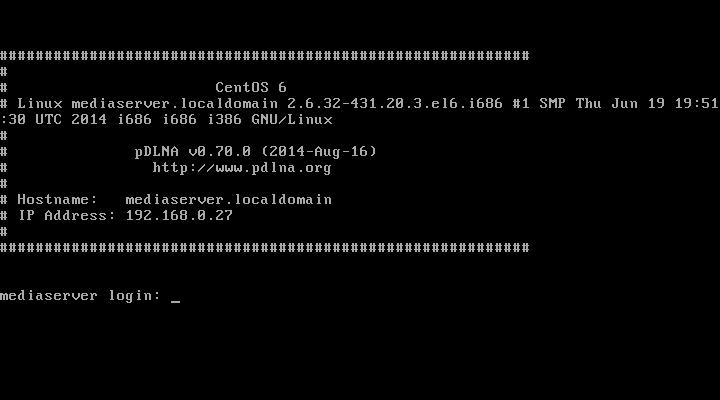
\includegraphics[width=34em]{images/vm_centos6_loginscreen}
	\label{fig:centos6-loginscreen}
	\caption{Boot-up screen of pre-installed CentOS 6 virtual machine image}
\end{figure}

\subsubsection{Changing the timezone}

In CentOS 6, all the available timezones are stored in the directory \verb|/usr/share/zoneinfo/|. Because of this, changing the timezone can be done via modifying the sysmlink for \verb|/etc/localtime| to the corresponding timezone file. An example is listed in the following snippet:

\begin{lstlisting}
pdlna@mediaserver:~$ sudo ln -sf /usr/share/zoneinfo/EST /etc/localtime
\end{lstlisting}

\subsubsection{Changing the keyboard layout}

In CentOS 6, all the available keyboard layouts are stored in the directory \verb|/lib/kbd/keymaps/i386|. Changing the keyboard layout can be done via modifying the \verb|KEYTABLE| key in the file \verb|/etc/sysconfig/keyboard| by opening the file with your favourite file editor:

\begin{lstlisting}
pdlna@mediaserver:~$ sudo vi /etc/sysconfig/keyboard
\end{lstlisting}

Additional documentation can be found here: \url{www.centos.org/docs/5/html/5.1/Deployment_Guide/s2-sysconfig-kybd.html}

\subsection{Debian GNU/Linux 7}

% apt-get install sudo openntpd git libfile-copy-recursive-perl
% vi /etc/sudoers

\subsubsection{Logon customization}

The logon customization, as can be seen in figure~\ref{fig:debian7-loginscreen}, is handeled by the script \verb|/etc/rc.local|, which was modified to call \verb|/usr/local/bin/update-issue.sh|, which updates the \verb|/etc/issue| and \verb|/etc/issue.net| files. The following three lines have also been added to this file, to delete sensitive data on startup:
\begin{colframefile}
\begin{verbatim}
/bin/rm -f /var/log/pdlna.log
/bin/rm -f /tmp/pdlna.db
/bin/rm -f /var/run/pdlna.pid
\end{verbatim}
\end{colframefile}

Additionally, the \verb|OpenSSH| server's configuration file (\verb|/etc/ssh/sshd_config|) has been modified to use the \verb|/etc/issue.net| file as a banner:
\begin{colframefile}
\begin{verbatim}
Banner /etc/issue.net
\end{verbatim}
\end{colframefile}

The \verb|/usr/local/bin/update-issue.sh| script can also be found on GitHub (\url{github.com/geuma/pDLNA-utils/blob/master/preinstalled-VMs/Debian7/update-issue.sh}).

\begin{figure}
	\centering
		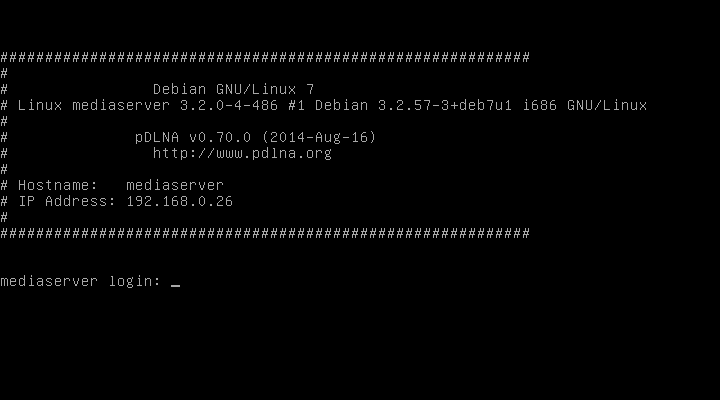
\includegraphics[width=34em]{images/vm_debian7_loginscreen}
	\label{fig:debian7-loginscreen}
	\caption{Boot-up screen of pre-installed Debian 7 virtual machine image}
\end{figure}

\subsubsection{Changing the timezone}

Changing the timezone in Debian GNU/Linux 7 can be done by executing the following command as a superuser and use its wizard to configure the correct timezone.

\begin{lstlisting}
pdlna@mediaserver:~$ sudo dpkg-reconfigure tzdata
\end{lstlisting}

\subsubsection{Changing the keyboard layout}

Changing the keyboard layout is as easy as changing the timezone. Just execute the following command as a superuser and use its wizard to configure the correct keyboard layout.

\begin{lstlisting}
pdlna@mediaserver:~$ sudo dpkg-reconfigure keyboard-configuration
\end{lstlisting}

\subsection{FreeBSD 9}

%shells/bash, security/sudo, devel/git, devel/p5-File-Copy-Recursive

\subsubsection{Logon customization}

The logon customization, as can be seen in figure~\ref{fig:freebsd9-loginscreen}, is handeled by the script \verb|/etc/rc.local|, which was created to call \verb|/usr/local/bin/update-issue.sh|, which updates the \verb|/etc/issue| and \verb|/etc/issue.net| files and delete sensitive data. The script \verb|/etc/rc.local| has been created with the following content and the executable bit has been set. By default, FreeBSD 9 executes this script at startup via \verb|/etc/rc.d/local|.
\begin{colframefile}
\begin{verbatim}
#!/bin/sh

/usr/local/bin/update-issue.sh
/bin/rm -f /var/log/pdlna.log
/bin/rm -f /tmp/pdlna.db
/bin/rm -f /var/run/pdlna.pid
\end{verbatim}
\end{colframefile}

Since the configuration file \verb|/etc/gettytab| is already configured to use the \verb|/etc/issue| file as a banner, no configuration to \verb|getty| was needed.

Additionally, the \verb|OpenSSH| server's configuration file (\verb|/etc/ssh/sshd_config|) has been modified to use the \verb|/etc/issue.net| file as a banner:
\begin{colframefile}
\begin{verbatim}
Banner /etc/issue.net
\end{verbatim}
\end{colframefile}

The \verb|/usr/local/bin/update-issue.sh| script can also be found on GitHub (\url{github.com/geuma/pDLNA-utils/blob/master/preinstalled-VMs/FreeBSD9/update-issue.sh}).

\begin{figure}
	\centering
		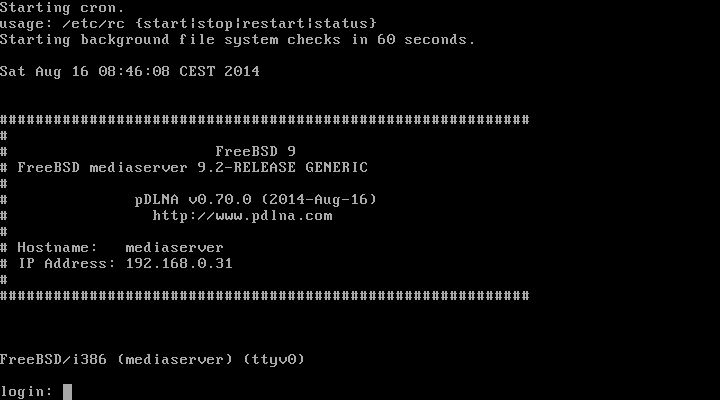
\includegraphics[width=34em]{images/vm_freebsd9_loginscreen}
	\label{fig:freebsd9-loginscreen}
	\caption{Boot-up screen of pre-installed FreeBSD 9 virtual machine image}
\end{figure}

\subsubsection{Changing the timezone}

In FreeBSD 9, all the available timezones are stored in the directory \verb|/usr/share/zoneinfo|. Because of this, changing the timezone can be done via copying the corresponding timezone file to \verb|/etc/localtime|. An example is listed in the following snippet:

\begin{lstlisting}
[pdlna@mediaserver ~]$ sudo copy /usr/share/zoneinfo/EST /etc/localtime
\end{lstlisting}

\subsubsection{Changing the keyboard layout}

Changing the keyboard layout is as easy as changing the timezone. Just execute the following command as a superuser and use its menu to configure the correct keyboard layout.

\begin{lstlisting}
[pdlna@mediaserver ~]$ sudo kbdmap
\end{lstlisting}

If you would like to change the keyboard layout in a persistent way, modify the file \verb|/etc/rc.conf|.